\PassOptionsToPackage{unicode=true}{hyperref} % options for packages loaded elsewhere
\PassOptionsToPackage{hyphens}{url}
\PassOptionsToPackage{dvipsnames,svgnames*,x11names*}{xcolor}
%
\documentclass[ignorenonframetext,]{beamer}
\usepackage{pgfpages}
\setbeamertemplate{caption}[numbered]
\setbeamertemplate{caption label separator}{: }
\setbeamercolor{caption name}{fg=normal text.fg}
\beamertemplatenavigationsymbolsempty
% Prevent slide breaks in the middle of a paragraph:
\widowpenalties 1 10000
\raggedbottom
\setbeamertemplate{part page}{
\centering
\begin{beamercolorbox}[sep=16pt,center]{part title}
  \usebeamerfont{part title}\insertpart\par
\end{beamercolorbox}
}
\setbeamertemplate{section page}{
\centering
\begin{beamercolorbox}[sep=12pt,center]{part title}
  \usebeamerfont{section title}\insertsection\par
\end{beamercolorbox}
}
\setbeamertemplate{subsection page}{
\centering
\begin{beamercolorbox}[sep=8pt,center]{part title}
  \usebeamerfont{subsection title}\insertsubsection\par
\end{beamercolorbox}
}
\AtBeginPart{
  \frame{\partpage}
}
\AtBeginSection{
  \ifbibliography
  \else
    \frame{\sectionpage}
  \fi
}
\AtBeginSubsection{
  \frame{\subsectionpage}
}
\usepackage{lmodern}
\usepackage{amssymb,amsmath}
\usepackage{ifxetex,ifluatex}
\usepackage{fixltx2e} % provides \textsubscript
\ifnum 0\ifxetex 1\fi\ifluatex 1\fi=0 % if pdftex
  \usepackage[T1]{fontenc}
  \usepackage[utf8]{inputenc}
  \usepackage{textcomp} % provides euro and other symbols
\else % if luatex or xelatex
  \usepackage{unicode-math}
  \defaultfontfeatures{Ligatures=TeX,Scale=MatchLowercase}
\fi
% use upquote if available, for straight quotes in verbatim environments
\IfFileExists{upquote.sty}{\usepackage{upquote}}{}
% use microtype if available
\IfFileExists{microtype.sty}{%
\usepackage[]{microtype}
\UseMicrotypeSet[protrusion]{basicmath} % disable protrusion for tt fonts
}{}
\IfFileExists{parskip.sty}{%
\usepackage{parskip}
}{% else
\setlength{\parindent}{0pt}
\setlength{\parskip}{6pt plus 2pt minus 1pt}
}
\usepackage{xcolor}
\usepackage{hyperref}
\hypersetup{
            pdftitle={Lecture 2 - Shortcomings of ad-hoc methods, complete case analysis, \& introduction to multiple imputation (MI)},
            pdfauthor={Jonathan Bartlett (thestatsgeek.com)},
            colorlinks=true,
            linkcolor=blue,
            filecolor=Maroon,
            citecolor=Blue,
            urlcolor=blue,
            breaklinks=true}
\urlstyle{same}  % don't use monospace font for urls
\newif\ifbibliography
\setlength{\emergencystretch}{3em}  % prevent overfull lines
\providecommand{\tightlist}{%
  \setlength{\itemsep}{0pt}\setlength{\parskip}{0pt}}
\setcounter{secnumdepth}{0}

% set default figure placement to htbp
\makeatletter
\def\fps@figure{htbp}
\makeatother


\title{Lecture 2 - Shortcomings of ad-hoc methods, complete case analysis, \&
introduction to multiple imputation (MI)}
\providecommand{\subtitle}[1]{}
\subtitle{Multiple imputation techniques for working with missing data}
\author{\href{https://thestatsgeek.com}{Jonathan Bartlett (thestatsgeek.com)}}
\date{Copenhagen, March 2020}

\begin{document}
\frame{\titlepage}

\begin{frame}
\tableofcontents[hideallsubsections]
\end{frame}
\hypertarget{ad-hoc-methods}{%
\section{Ad-hoc methods}\label{ad-hoc-methods}}

\begin{frame}{Ad-hoc methods}
\protect\hypertarget{ad-hoc-methods-1}{}

\begin{itemize}
\tightlist
\item
  Ad-hoc methods are simple and easy apparent solutions to handling
  missing data.
\item
  Commonly used examples are: simple mean imputation, missing category
  method, last observation carried forward.
\item
  All (except missing category) are examples of single imputation
  methods.
\item
  Question: in general will we get valid answers using these ad-hoc
  methods?
\end{itemize}

\end{frame}

\begin{frame}{Issues with ad-hoc methods}
\protect\hypertarget{issues-with-ad-hoc-methods}{}

\begin{itemize}
\tightlist
\item
  Answer: No in general.
\item
  They can introduce \textcolor{red}{bias} into estimates.
\item
  They can lead to confidence intervals that are too
  \textcolor{red}{narrow}.
\item
  The latter is true of all single imputation methods, unless special
  procedures are used to allow for uncertainty due to imputation
  (e.g.~bootstrapping)
\end{itemize}

\end{frame}

\begin{frame}{Simple mean imputation}
\protect\hypertarget{simple-mean-imputation}{}

\begin{itemize}
\tightlist
\item
  Replaces missing values with mean of observed.
\item
  Variance of the variable is artificially reduced.
\item
  Associations with other variables are distorted.
\item
  \textbf{It's a bad idea!}
\end{itemize}

\end{frame}

\begin{frame}{Regression mean imputation}
\protect\hypertarget{regression-mean-imputation}{}

\begin{itemize}
\tightlist
\item
  Replaces missing values with prediction based on observed variables.
\item
  Better than mean imputation.
\item
  Variance of the variable is still too small.
\item
  Associations with other variables may still be distorted.
\item
  \textbf{It's better, but still a bad idea!}
\end{itemize}

\end{frame}

\begin{frame}{Missing category method}
\protect\hypertarget{missing-category-method}{}

\begin{itemize}
\tightlist
\item
  For categorical variables with missing values, create a new missing
  category.
\item
  In general regression coefficients after using this method are biased.
\item
  To see why, think about the case where the variable is a
  confounder\ldots{}
\item
  An exception is with missing baseline in randomized trials, see (White
  and Thompson \protect\hyperlink{ref-Whiteux2fThompson:2005}{2005})
\end{itemize}

\end{frame}

\begin{frame}{Last observation carried forward (LOCF)}
\protect\hypertarget{last-observation-carried-forward-locf}{}

\begin{itemize}
\tightlist
\item
  In longitudinal studies, an approach that was historically popular is
  last observation carried forward (LOCF).
\item
  Makes strong, implausible assumptions.
\item
  In general neither conservative or liberal for treatment effects.
\item
  Bias depends on unknown treatment effect!
\item
  See (Molenberghs et al.
  \protect\hyperlink{ref-Molenberghsux2fThijs:2004}{2004}; Cook, Zeng,
  and Yi \protect\hyperlink{ref-Cookux2fZengux2fYi:2004}{2004};
  Carpenter et al.
  \protect\hyperlink{ref-Carpenterux2fKenwardux2fEvansux2fWhite:2004}{2004})
\end{itemize}

\end{frame}

\begin{frame}{Ad-hoc methods summary}
\protect\hypertarget{ad-hoc-methods-summary}{}

\begin{itemize}
\tightlist
\item
  Ad-hoc methods are an attempt to `solve' the problem of missing data.
\item
  They avoid any serious thinking about the issues raised by missing
  data.
\item
  They do not utilize statistical principles.
\item
  Generally they result in misleading conclusions.
\end{itemize}

\end{frame}

\hypertarget{complete-case-analysis}{%
\section{Complete case analysis}\label{complete-case-analysis}}

\begin{frame}{Complete case analysis}
\protect\hypertarget{complete-case-analysis-1}{}

\begin{itemize}
\tightlist
\item
  Complete case analysis (CCA) ignores all units/observations with
  incomplete data in those variables involved in analysis.
\item
  It is the default of most (all?!) statistical packages when presented
  with missing data.
\item
  We will lose precision in estimates (compared to full data).
\item
  We explore biases of CCA in different situations\ldots{}
\end{itemize}

\end{frame}

\begin{frame}{Marginal estimands}
\protect\hypertarget{marginal-estimands}{}

\begin{itemize}
\tightlist
\item
  Suppose we were interested in estimating the (marginal) mean systolic
  blood pressure (SBP) in a population.
\item
  The plot below shows the complete sample (n=1000) of SBP values:
\end{itemize}

\begin{center}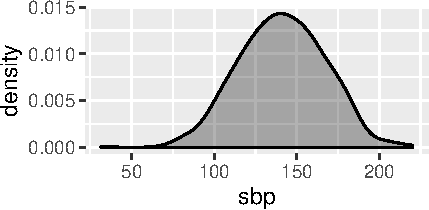
\includegraphics{Lecture2_files/figure-beamer/unnamed-chunk-2-1} \end{center}

The mean is 141.1

\end{frame}

\begin{frame}{MCAR - what will happen?}
\protect\hypertarget{mcar---what-will-happen}{}

\begin{itemize}
\tightlist
\item
  Now we will make 50\% of values missing.
\item
  If we make them missing completely at random, will the complete case
  distribution and mean go up or down?
\end{itemize}

\end{frame}

\begin{frame}{MCAR - what will happen?}
\protect\hypertarget{mcar---what-will-happen-1}{}

The complete case mean is 139.9

\begin{center}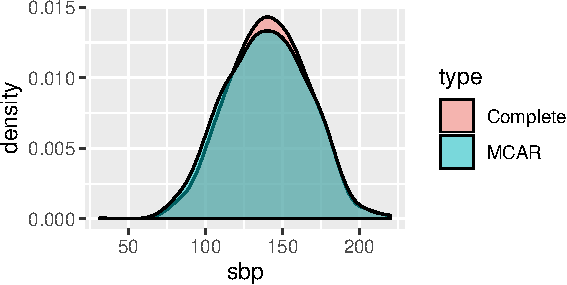
\includegraphics{Lecture2_files/figure-beamer/unnamed-chunk-4-1} \end{center}

\textbf{No bias}

\end{frame}

\begin{frame}{MNAR - what will happen?}
\protect\hypertarget{mnar---what-will-happen}{}

\begin{itemize}
\tightlist
\item
  Now we will make higher values of SBP more likely to be missing.
\item
  Will the complete case distribution and mean go up or down?
\end{itemize}

\end{frame}

\begin{frame}{MNAR - what will happen?}
\protect\hypertarget{mnar---what-will-happen-1}{}

The complete case mean is 125.6

\begin{center}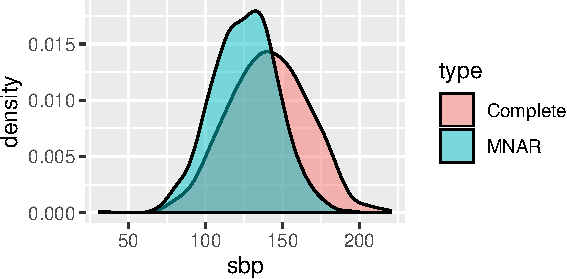
\includegraphics{Lecture2_files/figure-beamer/unnamed-chunk-6-1} \end{center}

\textbf{Biased downwards}

\end{frame}

\begin{frame}{MAR - what will happen?}
\protect\hypertarget{mar---what-will-happen}{}

\begin{itemize}
\tightlist
\item
  Now we will make values of SBP more likely to be missing if the
  person's age (assumed fully observed) is high.
\item
  Will the complete case distribution and mean go up or down?
\end{itemize}

\end{frame}

\begin{frame}{MAR - what will happen?}
\protect\hypertarget{mar---what-will-happen-1}{}

The complete case mean is 130.6

\begin{center}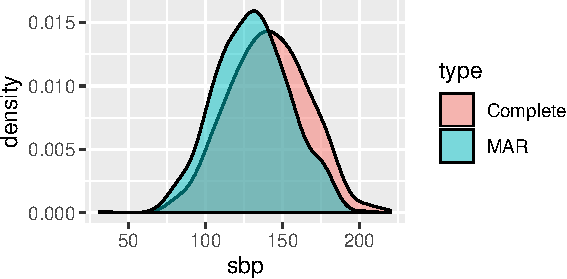
\includegraphics{Lecture2_files/figure-beamer/unnamed-chunk-8-1} \end{center}

\textbf{Biased downwards}

\end{frame}

\begin{frame}{Marginal estimands - conclusions}
\protect\hypertarget{marginal-estimands---conclusions}{}

\begin{itemize}
\tightlist
\item
  For marginal estimands like means, we get bias under both MAR and MNAR
  mechanisms.
\item
  Whether we get bias just depends on whether missingness is MCAR or
  not.
\item
  Since in practice MCAR often doesn't hold, CCA for marginal estimands
  will usually be biased.
\end{itemize}

\end{frame}

\begin{frame}{Complete case analysis - regression analyses}
\protect\hypertarget{complete-case-analysis---regression-analyses}{}

\begin{itemize}
\tightlist
\item
  Often we are interested in fitting a regression model for an outcome
  \(Y\) on covariates \(X_{1},..,X_{p}\).
\item
  A CCA drops any observations which have one or more values missing in
  the variables used in the regression.
\item
  With many variables in the regression and sporadic missingness, the
  complete cases can be a small subset, leading to big loss in
  information.
\item
  What about bias?
\end{itemize}

\end{frame}

\begin{frame}{Linear regression complete case analysis}
\protect\hypertarget{linear-regression-complete-case-analysis}{}

This is the full (complete) SBP against age data.

\begin{center}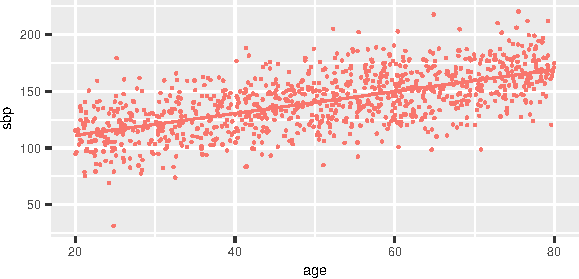
\includegraphics{Lecture2_files/figure-beamer/unnamed-chunk-9-1} \end{center}

\end{frame}

\begin{frame}{MCAR complete case regression}
\protect\hypertarget{mcar-complete-case-regression}{}

This is the CCA of the MCAR dataset.

\begin{center}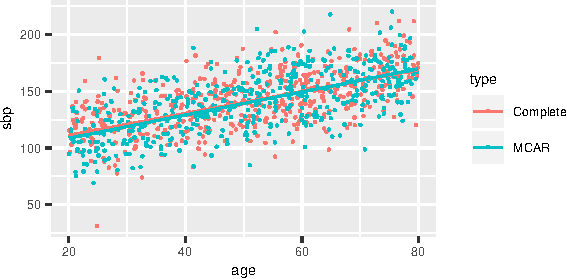
\includegraphics{Lecture2_files/figure-beamer/unnamed-chunk-10-1} \end{center}

CCA is unbiased, as we should expect.

\end{frame}

\begin{frame}{Missingness dependent on outcome}
\protect\hypertarget{missingness-dependent-on-outcome}{}

When missingness depends on outcome (SBP):

\begin{center}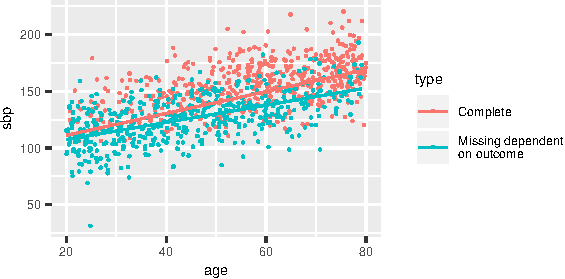
\includegraphics{Lecture2_files/figure-beamer/unnamed-chunk-11-1} \end{center}

CCA is now biased.

\end{frame}

\begin{frame}{Missingness dependent on covariate}
\protect\hypertarget{missingness-dependent-on-covariate}{}

When missingness depends on the covariate (age):

\begin{center}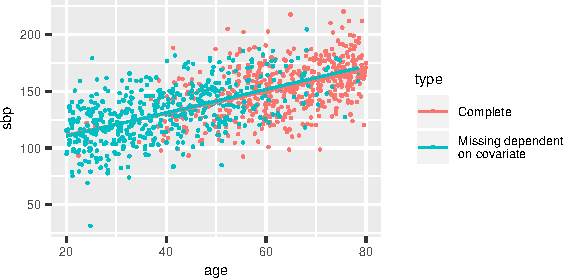
\includegraphics{Lecture2_files/figure-beamer/unnamed-chunk-12-1} \end{center}

CCA is unbiased.

\end{frame}

\begin{frame}{Complete case analysis - regression analyses}
\protect\hypertarget{complete-case-analysis---regression-analyses-1}{}

\begin{itemize}
\tightlist
\item
  CCA regression analyses are unbiased if probability of being a
  complete case is independent of outcome variable, conditional on
  covariates.
\item
  This condition doesn't related to which variable(s) (outcome or
  covariates) have missing values.
\item
  It is \textcolor{red}{not} true that CCA is valid under MAR and
  invalid under MNAR.
\item
  It can be valid under both types - the key is whether missingness is
  conditionally (on covariates) independent of outcome.
\end{itemize}

\end{frame}

\begin{frame}{Justification}
\protect\hypertarget{justification}{}

Why does this result hold in general?

\begin{itemize}
\tightlist
\item
  Let \(R\) denote whether a subject is a complete case (\(R=1\) for
  complete cases, \(R=0\) for incomplete cases)
\item
  Our assumption for missingness is that
  \(f(R|Y,\mathbf X)=f(R|\mathbf X)\)
\item
  A CCA involves fitting the conditional model for \(f(Y|\mathbf X)\) in
  the subset of subjects with \(R=1\): \[
  \begin{aligned}
  f(Y|\mathbf X,R=1) = \frac{f(Y,\mathbf X,R=1)}{f(\mathbf X,R=1)} &= \frac{f(R=1|\mathbf X,Y)f(\mathbf X,Y)}{f(R=1|\mathbf X)f(\mathbf X)} \\
    &= \frac{f(R=1|\mathbf X) f(\mathbf X,Y)}{f(R=1|\mathbf X) f(\mathbf X)} \\
    &= f(Y|\mathbf X)
  \end{aligned}
  \]
\item
  Thus the conditional distribution \(Y|X\) in the complete cases is the
  same as in the complete data.
\end{itemize}

\end{frame}

\begin{frame}{Complete case validity - Example}
\protect\hypertarget{complete-case-validity---example}{}

\begin{itemize}
\tightlist
\item
  (Bartlett et al. \protect\hyperlink{ref-Bartlett2014a}{2014}) reported
  results of an illustrative analysis based on cross-sectional data from
  the US NHANES 2003-2004 study.
\item
  They fitted a regression model for systolic blood pressure (SBP) with
  no. of alcoholic drinks, BMI, and age as covariates.
\item
  No.~of alcoholic drinks was missing for 34.1\% of individuals.
\item
  Missingness in this variable may well be related to level of alcohol
  consumption (i.e.~MNAR), age, (and maybe) BMI, but given these is
  probably unrelated to SBP.
\item
  If this assumption is true, the CCA is valid, even though the
  covariate is (assumed to be) MNAR.
\end{itemize}

\end{frame}

\begin{frame}{Logistic regression CCA}
\protect\hypertarget{logistic-regression-cca}{}

\begin{itemize}
\tightlist
\item
  If the outcome model is logistic regression, CCA can give valid
  estimates (of covariate effects) under even weaker missingness
  assumptions (Bartlett, Harel, and Carpenter
  \protect\hyperlink{ref-Bartlett2015}{2015}).
\item
  This is due to the symmetry property of odds ratios (the same reason
  we can use odds ratios in case-control studies).
\item
  For covariate effects (but not the intercept), we get consistent
  estimates if missingness is:

  \begin{itemize}
  \tightlist
  \item
    dependent on \(Y\), or
  \item
    dependent on \(\mathbf X=(X_{1},..,X_{p})\)
  \end{itemize}
\item
  Furthermore, missingness could be dependent on \(Y\) and
  \(X_{2},..,X_{p}\), and estimates of coefficient of \(X_{1}\) are
  still consistent.
\end{itemize}

\end{frame}

\begin{frame}{CCA - recommendations}
\protect\hypertarget{cca---recommendations}{}

\begin{itemize}
\tightlist
\item
  It is generally always a good idea to perform CCA for your analysis.
\item
  The estimates you get can be compared with those from other analyses
  which make other assumptions.
\item
  Important to remember that CCA might be valid in your situation,
  depending on the analysis you are performing and missingness
  assumptions.
\end{itemize}

\end{frame}

\begin{frame}{Why are we wasting our time on MAR and MNAR?}
\protect\hypertarget{why-are-we-wasting-our-time-on-mar-and-mnar}{}

\begin{itemize}
\tightlist
\item
  Validity of CCA doesn't fit neatly into the MCAR/MAR/MNAR framework.
\item
  Why then did we spend time defining and thinking about MAR and MNAR?
\item
  Answer: because an important collection of methods can give valid
  inferences under MAR mechanisms.
\item
  One such method is multiple imputation\ldots{}
\end{itemize}

\end{frame}

\hypertarget{multiple-imputation}{%
\section{Multiple imputation}\label{multiple-imputation}}

\begin{frame}{Multiple imputation}
\protect\hypertarget{multiple-imputation-1}{}

\begin{itemize}
\tightlist
\item
  Multiple imputation (MI) is a flexible and increasingly popular
  approach to handling missing data.
\item
  It relies (at least in its usual form) on assuming data are MAR.
\item
  We will introduce it in a simple setting with two variables.
\item
  Later we will look at extensions to more realistic situations.
\end{itemize}

\end{frame}

\begin{frame}{Intuition for MI}
\protect\hypertarget{intuition-for-mi}{}

\begin{itemize}
\tightlist
\item
  Suppose our data set has variables \(X\) and \(Y\), with some \(Y\)
  values MAR given \(X\).
\item
  Our aim is to impute missing values in \(Y\), taking \(X\) into
  account.
\item
  In parametric imputation, we specify a regression model for
  \(f(Y|X)\).
\item
  We want to impute the missing \(Y\) values from this model.
\item
  \textbf{$Y$ need not necessarily be the outcome in our final analysis}.
\end{itemize}

\end{frame}

\begin{frame}{Intuition for MI}
\protect\hypertarget{intuition-for-mi-1}{}

\begin{itemize}
\tightlist
\item
  MAR here means missingness in \(Y\) is independent of \(Y\), given
  \(X\).
\item
  This means that if we fit the model for \(f(Y|X)\) using complete
  cases, estimates are valid.
\item
  Using the fitted model, we can then impute \(Y\) for the incomplete
  cases.
\item
  With the imputed data set, we can calculate our statistic of interest
  (e.g.~sample mean, variance, regression of \(X\) on \(Y\)).
\end{itemize}

\end{frame}

\begin{frame}{Why multiple imputation?}
\protect\hypertarget{why-multiple-imputation}{}

In multiple imputation we create a number \(M\) imputed datasets,
estimate our parameter(s) of interest from each imputed dataset, and
then calculate the average across imputations

There are two main reasons why we create \emph{multiple} imputed
datasets:

\begin{enumerate}
\tightlist
\item
  We reduce Monte-Carlo error which is introduced through using a
  simulation based method
\item
  Estimating variances and finding confidence intervals is relatively
  easy if we create multiple imputations, but is rather difficult with
  only a single imputation
\end{enumerate}

\end{frame}

\begin{frame}{Multiple imputation for one continuous variable}
\protect\hypertarget{multiple-imputation-for-one-continuous-variable}{}

\begin{itemize}
\tightlist
\item
  Next describe the details/steps for linear regression imputation of
  one variable.
\item
  Later on, we will see that application of MI in practice requires
  careful considerations of a number of aspects (e.g.~missingness
  assumptions, model specification).
\item
  For now, we will put these to one side.
\end{itemize}

\end{frame}

\begin{frame}{Multiple imputation for one continuous variable}
\protect\hypertarget{multiple-imputation-for-one-continuous-variable-1}{}

\begin{itemize}
\tightlist
\item
  \(X\) is fully observed.
\item
  \(Y\) contains missing values, and we assume \(Y\) is MAR given \(X\).
\item
  We want to create multiple imputations of the missing values in \(Y\),
  using \(X\).
\item
  We will create \(M\) imputations - we will come back to the choice of
  \(M\) later.
\end{itemize}

\end{frame}

\begin{frame}{The observed data}
\protect\hypertarget{the-observed-data}{}

The plot shows the complete cases (where \(Y\) and \(X\) observed) and
five subjects with \(X\) observed but \(Y\) missing.

\begin{center}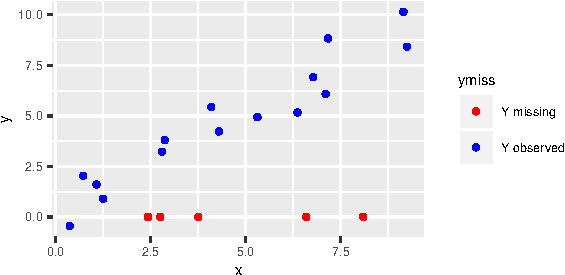
\includegraphics{Lecture2_files/figure-beamer/unnamed-chunk-14-1} \end{center}

\end{frame}

\begin{frame}{Step 1 - fit the imputation model}
\protect\hypertarget{step-1---fit-the-imputation-model}{}

We first fit the imputation model.

This is a model for the partially observed variable (\(Y\)) on the fully
observed variable (\(X\)), using a CCA.

\begin{center}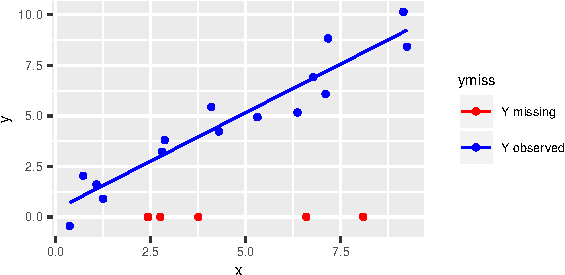
\includegraphics{Lecture2_files/figure-beamer/unnamed-chunk-15-1} \end{center}

\end{frame}

\begin{frame}{Step 2 - draw new imp. model parameter values}
\protect\hypertarget{step-2---draw-new-imp.-model-parameter-values}{}

Next we perturb the fitted line to account for uncertainty in its
estimation (we take draws from the Bayesian posterior of the regression
model parameters).

\begin{center}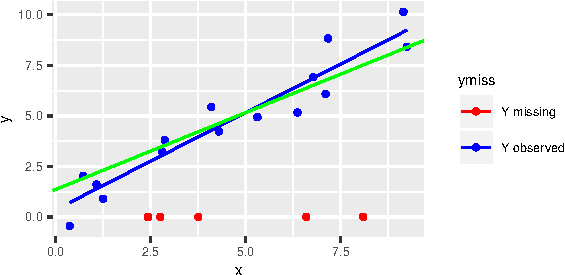
\includegraphics{Lecture2_files/figure-beamer/unnamed-chunk-17-1} \end{center}

\end{frame}

\begin{frame}{Step 3 - calculate predicted values}
\protect\hypertarget{step-3---calculate-predicted-values}{}

We then calculate predicted value of \(Y\) for those with \(Y\) missing.

\begin{center}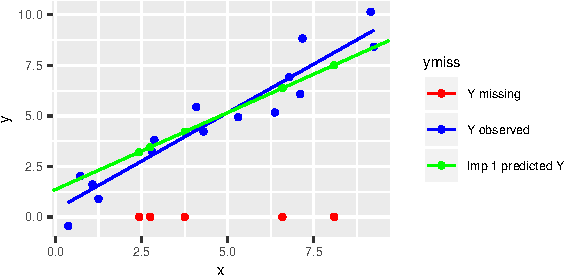
\includegraphics{Lecture2_files/figure-beamer/unnamed-chunk-19-1} \end{center}

\end{frame}

\begin{frame}{Step 4 - create imputed values}
\protect\hypertarget{step-4---create-imputed-values}{}

Imputed values are random draws centred at predicted \(Y\) values, with
error variance as drawn in earlier Bayesian posterior draw step.

\begin{center}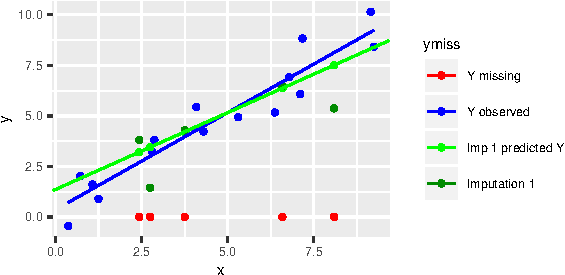
\includegraphics{Lecture2_files/figure-beamer/unnamed-chunk-21-1} \end{center}

\end{frame}

\begin{frame}{Step 5 - repeat steps to create more imputations}
\protect\hypertarget{step-5---repeat-steps-to-create-more-imputations}{}

We then repeat these steps to create as many imputations as desired:

\begin{itemize}
\tightlist
\item
  draw new parameter values from Bayesian posterior
\item
  draw new predicted values
\item
  draw new imputations around predicted values
\end{itemize}

\begin{center}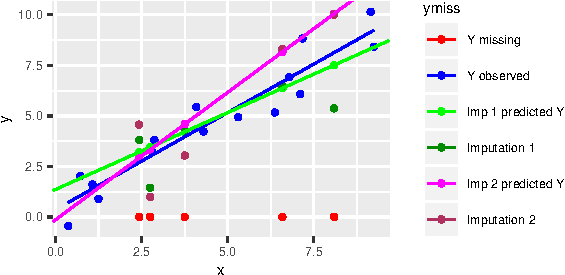
\includegraphics{Lecture2_files/figure-beamer/unnamed-chunk-23-1} \end{center}

\end{frame}

\begin{frame}{Algorithm}
\protect\hypertarget{algorithm}{}

\begin{itemize}
\tightlist
\item
  Estimate \(\sigma^{2},\beta_{0},\beta_{1}\) using the \(n_{0}\)
  complete case analysis, giving
  \(\hat{\sigma}^{2},\hat{\beta}_{0},\hat{\beta}_{1}\).
\item
  For \(m=1,..,M\)
\item
  Draw from posterior distribution of parameters:

  \begin{enumerate}
  \tightlist
  \item
    Draw a \(\sigma^{2(m)}\) from
    \(\hat\sigma^2 (n_0-2) / \chi^2_{n_0-2}.\)
  \item
    Draw \((\beta^{m}_0,\beta^{m}_1)\) from \[N \left\{ 
      \begin{pmatrix}\hat\beta_0 \\\hat\beta_1 \end{pmatrix},
      \sigma^{2(m)} (W^TW)^{-1} \right\}
      \]
  \end{enumerate}
\item
  If \(Y\) is missing for subject \(i\), impute \(Y_{i}\) by \[
  Y^{m}_{i} = \beta^{m}_{0} + \beta^{m}_{1} X_{i} + \epsilon^{m}_{i}
  \] where \(\epsilon^{m}_{i} \sim N(0, \sigma^{2(m)})\)
\end{itemize}

\end{frame}

\begin{frame}{Things to note}
\protect\hypertarget{things-to-note}{}

\begin{itemize}
\tightlist
\item
  Imputations are constructed by adding normal errors to the predicted
  value of \(Y\) based on the value of \(X\).
\item
  The variance of these errors depends on the estimated error variance
  in the model fitted to the complete cases.
\item
  For a given value of \(X\), the predicted values are different for
  each imputation, because a different line is used for each imputation.
\item
  The new imputation model parameter values are draws from their
  posterior distribution, under standard non-informative priors.
\end{itemize}

\end{frame}

\begin{frame}{Imputation using other types of model}
\protect\hypertarget{imputation-using-other-types-of-model}{}

\begin{itemize}
\tightlist
\item
  Imputation can also be performed using other types of regression
  model.
\item
  These can be chosen so that they are suitable for the variable being
  imputed.
\item
  e.g.~logistic regression for binary variables.
\item
  The principles outlined remain the same.
\item
  The only changes are that we take a draw from a different distribution
  depending on the type of regression model.
\end{itemize}

\end{frame}

\begin{frame}{Analysis of imputed datasets}
\protect\hypertarget{analysis-of-imputed-datasets}{}

\begin{itemize}
\tightlist
\item
  As described above, we have imputed \(M\) complete data sets.
\item
  We analyse each of them in the usual way (i.e.~using the model
  intended for the complete data) giving us \(M\) estimates of the
  original quantity of interest, say \(\theta.\) Denote these estimates
  \(\hat\theta_1,\dots,\hat\theta_M.\)
\item
  The analysis of each imputed data set will also give an estimate of
  the variance of the estimate \(\hat\theta_m,\) say \(\hat\sigma^2_m.\)
  Again, this is the usual variance estimate from the model.
\item
  We combine these quantities to get our overall estimate and its
  variance using certain rules, developed by Rubin.
\end{itemize}

\end{frame}

\begin{frame}{Combining the estimates - Rubin's rules}
\protect\hypertarget{combining-the-estimates---rubins-rules}{}

Let the multiple imputation estimate of \(\theta\) be
\(\hat\theta_{MI}.\) Then

\[\hat\theta_{MI} =\frac{1}{M} \sum_{m=1}^M \hat\theta_m.\]

Further define the within imputation and between imputation components
of variance by
\[\hat\sigma^2_w = \frac{1}{M} \sum _{m=1}^M \hat\sigma^2_m,\quad\mbox{ and } \quad \hat\sigma^2_b = \frac{1}{M-1} \sum_{m=1}^M (\hat\theta_m - \hat\theta_{MI} )^2,\]
Then
\[\hat\sigma^2_{MI} =  \left( 1 + \frac{1}{M} \right) \hat\sigma^2_b + \hat\sigma^2_w,\]
so the estimated standard error of \(\hat\theta_{MI}\) is
\(\hat\sigma_{MI}.\)

\end{frame}

\begin{frame}{Inference for \(\theta\)}
\protect\hypertarget{inference-for-theta}{}

To test the null hypothesis \(\theta=\theta_0,\) compare
\[ \frac{\hat\theta_{MI} - \theta_0}{\hat\sigma_{MI}} \mbox{\quad to \quad} t_\nu,\]
where
\[\nu = (M-1) \left[ 1 + \frac{ \hat\sigma^2_w}{(1 + 1/M)\hat\sigma^2_b}\right]^2.\]
Thus, if \(t_{\nu,0.975}\) is the 97.5\% point of the \(t\) distribution
with \(\nu\) degrees of freedom, the 95\% confidence interval is
\[(\hat\theta_{MI}-\hat\sigma_{MI} t_{\nu,0.975},\quad \hat\theta_{MI}+\hat\sigma_{MI} t_{\nu,0.975})\]

\end{frame}

\begin{frame}{Software}
\protect\hypertarget{software}{}

\begin{itemize}
\tightlist
\item
  As we shall see, the software automates the previous steps.
\item
  Although these steps are fairly automated, our input is critical.
\item
  There are various modelling choices to be made, and poor choices can
  lead to invalid inferences.
\end{itemize}

\end{frame}

\begin{frame}{The attractions of MI}
\protect\hypertarget{the-attractions-of-mi}{}

\begin{itemize}
\tightlist
\item
  MI is attractive, because once we have imputed the missing data, we
  can analyse the completed data sets as we would have done if no data
  were missing.
\item
  It is particularly useful in messy complex datasets, with missing
  values in multiple variables, where alternative approaches are less
  readily applied.
\item
  Compared to CCA, MI can often give estimates with improved precision.
\end{itemize}

\end{frame}

\begin{frame}{When is MI is the same as complete case analysis?}
\protect\hypertarget{when-is-mi-is-the-same-as-complete-case-analysis}{}

\begin{itemize}
\tightlist
\item
  If missingness is only in the outcome, and the analysis model is the
  same as the imputation model (i.e.~no auxiliary variables), MI gives
  you (essentially) the same estimates as complete case analysis.
\item
  So in this special case, there is no point in doing MI.
\end{itemize}

\end{frame}

\begin{frame}{Likelihood based analyses}
\protect\hypertarget{likelihood-based-analyses}{}

\begin{itemize}
\tightlist
\item
  Also note that some methods (e.g.~linear mixed models) analyse all
  observed data using maximum likelihood.
\item
  They are valid under MAR, and are efficient.
\item
  e.g.~in longitudinal trials with missingness in outcomes, there may be
  no need to do MI.
\item
  But MI can incorporate auxiliary variables, which is often very
  useful.
\end{itemize}

\end{frame}

\begin{frame}{Some papers on MI}
\protect\hypertarget{some-papers-on-mi}{}

(Schafer \protect\hyperlink{ref-Schafer:1999}{1999})

(Buuren \protect\hyperlink{ref-Buuren:2007}{2007})

(Kenward and Carpenter
\protect\hyperlink{ref-Kenwardux2fCarpenter:2007}{2007})

(Sterne et al.
\protect\hyperlink{ref-Sterneux2fWhiteux2fCarlin:2009}{2009})

There are of course many many more\ldots{}

\end{frame}

\begin{frame}{Some books on missing data and MI}
\protect\hypertarget{some-books-on-missing-data-and-mi}{}

Statistical Analysis with Missing Data (Little and Rubin
\protect\hyperlink{ref-little2019statistical}{2019}) -- excellent book
on analysis with missing data. 3rd edition recently released.

Flexible Imputation of Missing Data (Van Buuren
\protect\hyperlink{ref-van2018flexible}{2018}) -- A particular focus on
\href{https://cran.r-project.org/web/packages/mice/index.html}{mice}
package in R. 2nd edition recently release. Free online version
\href{https://stefvanbuuren.name/fimd/}{here}

Multiple Imputation and its Application (Carpenter and Kenward
\protect\hyperlink{ref-CarpenterKenward2013}{2013}) -- includes coverage
of imputation with survival data, multi-level data, non-linearities and
interactions, sensitivity analyses.

\end{frame}

\begin{frame}{Summary}
\protect\hypertarget{summary}{}

\begin{itemize}
\tightlist
\item
  Ad-hoc methods attempt to deal with the computational difficulty
  introduced by missing data.
\item
  But they generally do not give valid inferences under plausible
  assumptions.
\item
  MI gives valid inferences if data are MAR and the imp. model is
  correctly specified.
\item
  So far though we have only considered the case of a single partially
  observed continuous variable.
\item
  In the next session we will explore its extension to more realistic
  settings.
\end{itemize}

\end{frame}

\begin{frame}[allowframebreaks]{References}
\protect\hypertarget{references}{}

\hypertarget{refs}{}
\leavevmode\hypertarget{ref-Bartlett2014a}{}%
Bartlett, J W, J R Carpenter, K Tilling, and S Vansteelandt. 2014.
``Improving upon the efficiency of complete case analysis when
covariates are MNAR.'' \emph{Biostatistics} 15: 719--30.

\leavevmode\hypertarget{ref-Bartlett2015}{}%
Bartlett, J W, O Harel, and J R Carpenter. 2015. ``Asymptotically
Unbiased Estimation of Exposure Odds Ratios in Complete Records Logistic
Regression.'' \emph{American Journal of Epidemiology} 182 (8): 730--36.

\leavevmode\hypertarget{ref-Buuren:2007}{}%
Buuren, S van. 2007. ``Multiple Imputation of Discrete and Continuous
Data by Fully Conditional Specification.'' \emph{Statistical Methods in
Medical Research} 16: 219--42.

\leavevmode\hypertarget{ref-Carpenterux2fKenwardux2fEvansux2fWhite:2004}{}%
Carpenter, J, M Kenward, S Evans, and I White. 2004. ``Letter to the
editor: Last observation carry forward and last observation analysis by
J.~Shao and B. Zhong, Statistics in Medicine, 2003, \textbf{22},
2429--2441.'' \emph{Statistics in Medicine} 23: 3241--4.

\leavevmode\hypertarget{ref-CarpenterKenward2013}{}%
Carpenter, J R, and M G Kenward. 2013. \emph{Multiple Imputation and its
Application}. John Wiley \& Sons, Ltd, Chichester, U.K.

\leavevmode\hypertarget{ref-Cookux2fZengux2fYi:2004}{}%
Cook, R J, L Zeng, and G Y Yi. 2004. ``Marginal analysis of incomplete
longitudinal binary data; a cautionary note on LOCF imputation.''
\emph{Biometrics}, 820--28.

\leavevmode\hypertarget{ref-Kenwardux2fCarpenter:2007}{}%
Kenward, M G, and J R Carpenter. 2007. ``Multiple Imputation: Current
Perspectives.'' \emph{Statistical Methods in Medical Research} 16:
199--218.

\leavevmode\hypertarget{ref-little2019statistical}{}%
Little, Roderick JA, and Donald B Rubin. 2019. \emph{Statistical
Analysis with Missing Data}. Vol. 793. John Wiley \& Sons.

\leavevmode\hypertarget{ref-Molenberghsux2fThijs:2004}{}%
Molenberghs, G, H Thijs, I Jansen, C Beunkens, M G Kenward, C
Mallinkrodt, and R J Carroll. 2004. ``Analyzing Incomplete Longitudinal
Clinical Trial Data.'' \emph{Biostatistics} 5: 445--64.

\leavevmode\hypertarget{ref-Schafer:1999}{}%
Schafer, J L. 1999. ``Multiple imputation: a primer.'' \emph{Statistical
Methods in Medical Research} 8: 3--15.

\leavevmode\hypertarget{ref-Sterneux2fWhiteux2fCarlin:2009}{}%
Sterne, J A C, I R White, J B Carlin, M Spratt, P Royston, M G Kenward,
A M Wood, and J R Carpenter. 2009. ``Multiple imputation for missing
data in epidemiological and clinical research: potential and pitfalls.''
\emph{British Medical Journal} 339: 157--60.

\leavevmode\hypertarget{ref-van2018flexible}{}%
Van Buuren, Stef. 2018. \emph{Flexible Imputation of Missing Data}.
Chapman; Hall/CRC.

\leavevmode\hypertarget{ref-Whiteux2fThompson:2005}{}%
White, I R, and S G Thompson. 2005. ``Adjusting for Partially Missing
Baseline Measurements in Randomized Trials.'' \emph{Statistics in
Medicine} 24: 993--1007.

\end{frame}

\end{document}
